José Santos y Ángel Monteagudo presentan una serie de experimentos para estudiar
las propiedades, características y comportamiento del autómata celular.

En esta sección, se presentan los experimentos más relevantes que se presentan
en el artículo, así como, también sus resultados. Para ello, se utiliza una rejilla
de $125.000$ celdas, es decir, $50^3$ al tener tres dimensiones.

\section{Influencia del parámetro \textit{Tasa de mutación base (m)}}

De cara a estudiar la capacidad del autómata celular para generar diferentes comportamientos,
los autores realizaron tres experimentos en los que se presenta una configuración de parámetros
locales por defecto, es decir, como se muestra en la tabla 6.1. En cada experimento, la
única variación se encuentra en el parámetro \textit{tasa de mutación base (m)}. Respecto al
número de iteraciones en este conjunto de experimento los autores realizan $1.000$ iteraciones en
cada caso, y siempre comienza con una única célula sana en el centro de la rejilla.

\begin{table}[h!]
  \centering
  \caption{Valores de los parámetros, excepto \textit{m}.}
  \label{tab:table1}
  \begin{tabular}{ccc}
    \toprule
    Nombre & Símbolo & Valor\\
    \midrule
    Tamaño del telómero & tl & 50\\
    Muerte por daño genético & e & 10\\
    Factor de incremento de tasa de mutación base & i & 100\\
    Muerte de un vecino & g & 30\\
    Muerte aleatoria & a & 1000\\
    \bottomrule
  \end{tabular}
\end{table}

Este parámetro influye en la probabilidad de que aparezcan nuevas mutaciones durante
el proceso de división celular o mitosis. La probabilidad viene dada por la fórmula
$1/m$, por lo que un valor grande de $m$ dará una probabilidad más baja de que
aparezca una nueva mutación en cada célula en cada evento mitótico que haya pasado
las pruebas.

A continuación, se muestra cada uno de los experimentos (media de realizar 5 veces cada experimento) especificando en cada caso
el valor $m$ utilizado, mostrando tres gráficas: una primera gráfica que muestra la
evolución de las células cancerosas frente a las células sanas; una segunda gráfica que
muestra el número de células que contiene qué marcador o marcadores del cáncer.

\subsection{Experimento 1: Tasa de mutación base igual a 10.000}

En este primer experimento, los autores presentan un valor para el parámetro
tasa de mutación base de $m=10.000$. Realizan una simulación de $1.000$ iteraciones.

\begin{figure}[h]
\centering
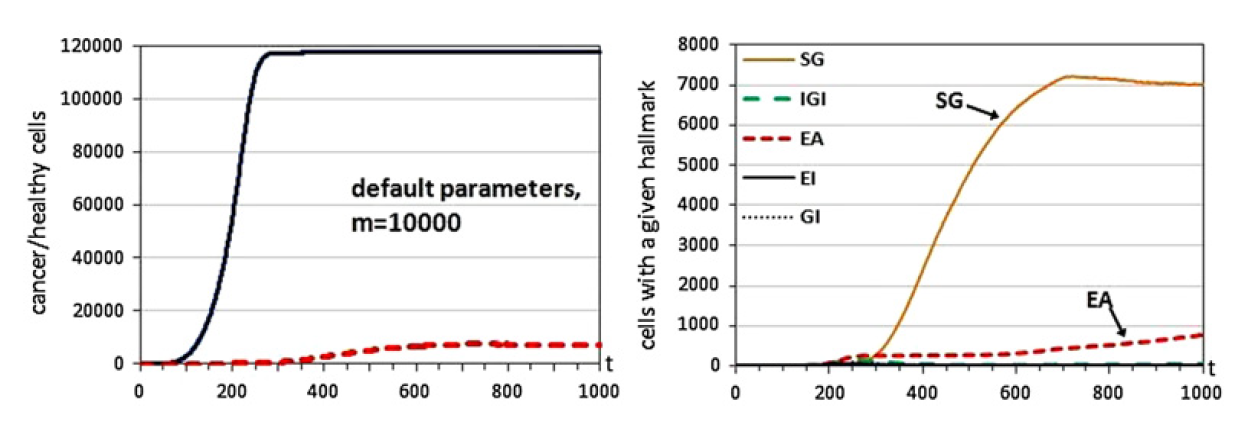
\includegraphics[scale=0.6]{figures/experiments/exp1}
\caption{Resultados obtenidos por los autores para el experimento con $m=10,000$.}
\label{fig:exp1}
\end{figure}

En la figura~\ref{fig:exp1} se presentan los resultados obtenidos tras la ejecución de la
simulación. Aquí, la tasa de mutación base hace que la probabilidad de que suceda una
mutación durante la mitosis sea especialmente baja.

El número de células cancerosas no presenta una proliferación destacada, y tiende a
mantenerse constante debido a que actúan determinados mecanismos sobre este tipo de células,
por ejemplo, la apoptosis.

Observando la gráfica que presenta los marcadores más relevantes se observa como
$SG$ toma ventaja. Este marcador permite a la célula falsificar los mensajes de
división celular y realizar así la mitosis. Esto ocurre porque este tipo de células
encuentra vía libre para proliferar en la zona exterior de la rejilla, debido a que
en ese lugar las células sanas no pueden proliferar por no disponer de suficiente
factor de crecimiento, lo que provoca que encuentre espacio libre.

El marcador $EA$ permite a la célula evadir la apoptosis, las cuales escapan
a los controles que presenta el cuerpo contra el cáncer. Esas células tienden a
permanecer en el centro de la rejilla, e incluso, a proliferar si no se encuentran con
algún otro límite, como por ejemplo, la falta de espacio.

El resto de marcadores no tienen presencia o su número es despreciable.

\subsection{Experimento 2: Tasa de mutación base igual a 1.000}

En el segundo experimento, los autores alteran el valor para el parámetro tasa de
mutación base a $m=1.000$. Esto es, una mayor probabilidad de que ocurran mutaciones
durante la mitosis.

\begin{figure}[h]
\centering
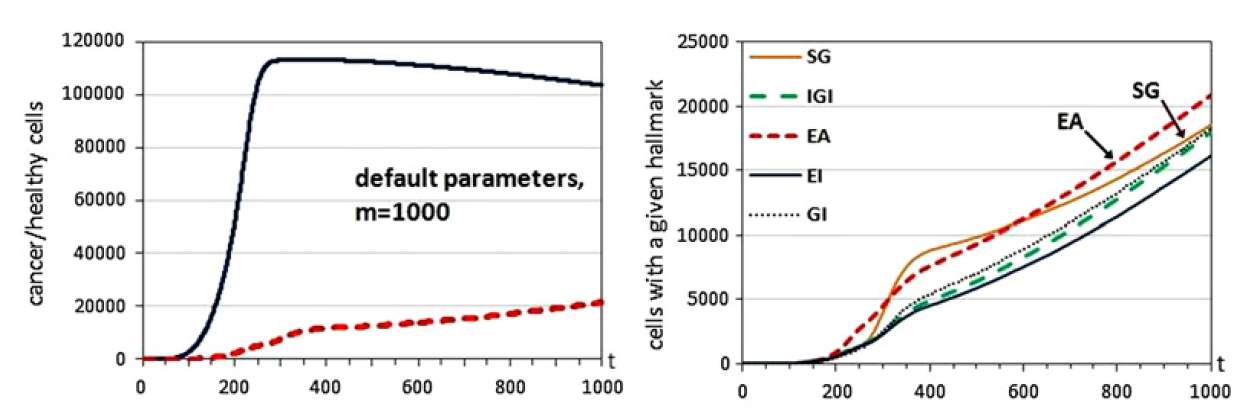
\includegraphics[scale=0.6]{figures/experiments/exp2}
\caption{Resultados obtenidos por los autores para el experimento con $m=1.000$.}
\label{fig:exp2}
\end{figure}

En la figura~\ref{fig:exp2} se muestran las mismas dos gráficas que en el experimento anterior.
En la primera de ellas, se observa como al finalizar la simulación el número de células
cancerosas es mayor, en torno al doble que en el experimento anterior.

En cuanto a los marcadores presentes, en este caso se dan todos los marcadores, aumentan en
número durante la simulación. El marcador $SG$ toma cierta ventaja, aunque se ve superado por
otros que se comentan a continuación, por el mismo motivo que en el experimento anterior. El
marcador más relevante al finalizar la simulación es $EA$. Esto contribuye a evadir
los mecanismo de proliferación, junto a la presencia del marcador $IGI$, el cual
provoca con una probabilidad dada la muerte de una célula sana para ser reemplazada por
la célula hija resultante. Esto último, provoca la proliferación mayor en el centro
de la rejilla, ya que las células pueden saltarse los límites mayores que se dan en ese lugar.

El resto de marcadores no son especialmente relevantes en esta simulación, como se podrá comprobar
en experimentos posteriores.

\subsection{Experimento 3: Tasa de mutación base igual a 100}

En este tercer, y último experimento, se presenta un experimento con una probabilidad de obtención de
mutaciones durante la mitosis mayor que en los dos anteriores.

\begin{figure}[h]
\centering
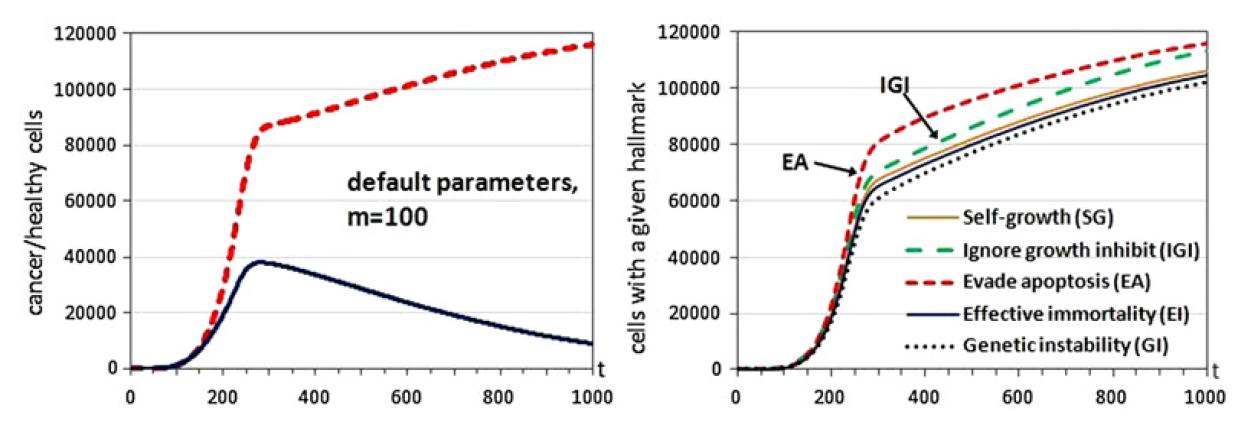
\includegraphics[scale=0.6]{figures/experiments/exp3}
\caption{Resultados obtenidos por los autores para el experimento con $m=100$.}
\label{fig:exp3}
\end{figure}

En la figura~\ref{fig:exp3}, se observa como en la primera parte de la simulación la proliferación
de las células cancerosas es mayor, llegando a suponer casi la totalidad de las células presentes
al finalizar la simulación.

En cuanto a los marcadores, los dos marcadores más relevantes son $EA$ e $IGI$, los cuales
permiten la proliferación en el centro de la rejilla, como se ha descrito anteriormente.
El resto, aunque están presentes, no son especialmente relevantes, y se obtienen debido a
los siguientes dos factores:

\begin{itemize}
  \item Las mutaciones son adquiridas de forma aleatoria en una célula, por tanto hay células localizadas aleatoriamente con algún marcador adquirido.
  \item Cuando una célula adquiere un marcador, como el marcador IGI, puede proliferar en su entorno inmediato (donde las nuevas células pueden adquirir nuevos marcadores durante la división), así que hay clústeres de concentraciones o células localizadas con los marcadores adquiridos.
\end{itemize}

\section{Influencia del resto de parámetros}

Para comprobar la influencia del resto de parámetros que intervienen en la simulación,
los autores realizan una modificación de los mismos. En la tabla 6.2 se muestran los valores
utilizados en esta ocasión, alterando el tamaño del telómero ($tl$), lo que supone
menos oportunidades de división de la célula original y de sus descendientes, entre otros
cambios.

\begin{table}[h!]
  \centering
  \caption{Valores de los parámetros.}
  \label{tab:table1}
  \begin{tabular}{ccc}
    \toprule
    Nombre & Símbolo & Valor\\
    \midrule
    Tasa de mutación base & m & 100.000\\
    Tamaño del telómero & tl & 35\\
    Muerte por daño genético & e & 20\\
    Factor de incremento de tasa de mutación base & i & 100\\
    Muerte de un vecino & g & 10\\
    Muerte aleatoria & a & 400\\
    \bottomrule
  \end{tabular}
\end{table}

Las pruebas anteriores sirven para comprobar la dificultad de aparición del cáncer en
función del parámetro $m$. La configuración inicial es la misma que en los experimentos
anteriores, exceptuando el número de iteraciones, que en este caso asciende a $5.000$

\begin{figure}[h]
\centering
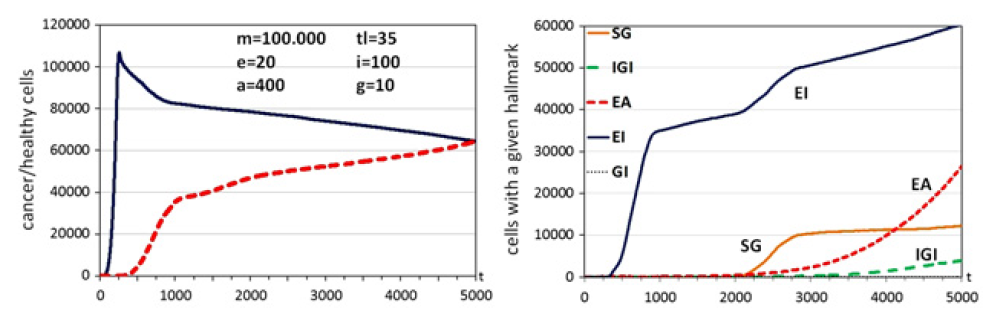
\includegraphics[scale=0.8]{figures/experiments/exp4}
\caption{Resultado de la simulación para comprobar la influencia del resto de parámetros.}
\label{fig:exp4}
\end{figure}

En la figura~\ref{fig:exp4} se presentan las mismas dos gráficas. La primera muestra como
al finalizar la simulación se dan el mismo números de células cancerosas que sanas, por
lo que el tumor ha proliferado antes de finalizar. Esto se explica, entre otros, por
un menor valor de $tl$, lo que provoca que aparezcan huecos libres en el centro que
permiten la proliferación de las células cancerosas.

En cuanto a los marcadores, $EI$ toma una gran ventaja respecto al resto. Debido, también,
a un menor valor de $tl$, este marcador permite la progresión del cáncer incluso con un tamaño de telómero igual a $0$.

El siguiente marcador que toma ventaja al finalizar la simulación es $EA$. Aparece sobre la iteración 2000,
por lo que las células que adquieren este marcador permite que las células cancerosas incrementen en número
al permitirles evadir el límite que existe por daño genético.

El marcador $IGI$ no prolifera rápidamente como en el caso previo, porque ahora hay más sitios vacantes
porque muchas más células han muerto por alcanzar el número límite de divisiones y han dejado hueco,
junto a una mayor tasa de muerte aleatoria por el parámetro $a$.

Por último, el marcador $SG$ prolifera fuera del límite espacial replicativo, como
se ha observado en los experimentos anteriores.

\section{Influencia de parámetros con rejilla completa de células sanas}

En este caso, se parte con una rejilla completa de células sanas. En cuanto a los parámetros,
se utilizan los mismos que en la secciones anteriores. Primero una simulación de $8.000$ iteraciones
con los parámetros por defecto, y luego una segunda de $100.000$ iteraciones con los parámetros
utilizados en el experimento de la figura~\ref{fig:exp4}.

En este caso, la simulación se corresponde con una equivalencia temporal
de $2.3$ años y $29.7$ años respectivamente.

\begin{figure}[h]
\centering
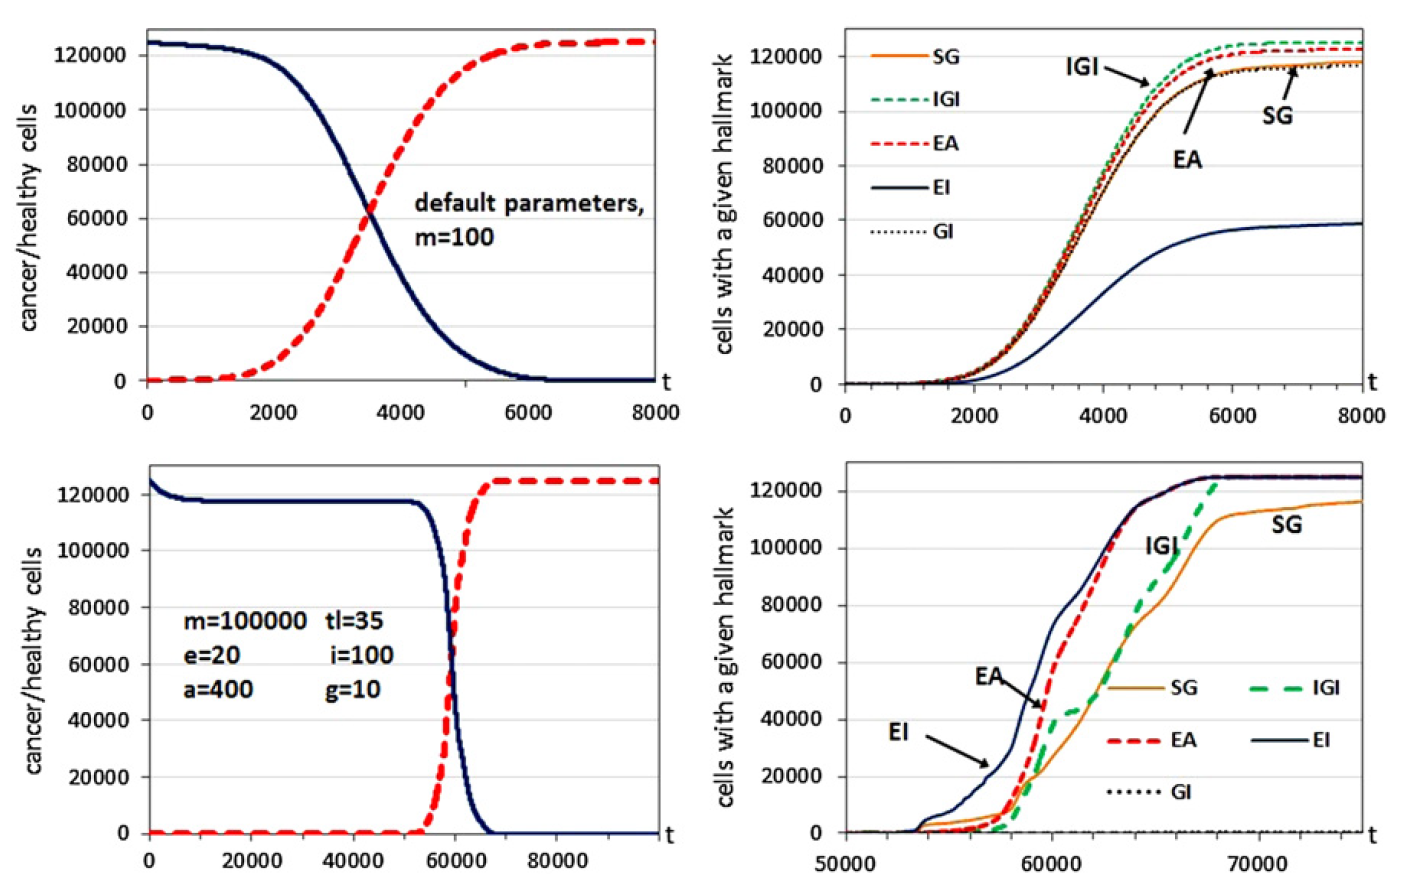
\includegraphics[scale=0.5]{figures/experiments/exp5}
\caption{Resultado de la simulación para comprobar la influencia del resto de parámetros con rejilla completa de células sanas.}
\label{fig:exp5}
\end{figure}

En el primer caso, es importante la aparición del marcador $IGI$ ya que no existe espacio
para proliferar en el centro de la rejilla. El siguiente marcador, por relevancia, es $EA$
el cual permite la proliferación evitando otro límite por apoptosis.

El marcador $GI$ permite la aparición de más mutaciones en las células durante la mitosis, por ello,
se acumulan más mutaciones que no son relevante en esta primera simulación.

En el segundo caso, el marcador $EI$ toma ventaja debido a que permite saltarse el límite por un
menor valor de $tl$, combinado a marcadores como $IGI$ o $EA$ se obtiene una proliferación mayor del
tumor.

El resto de mutaciones no son especialmente relevantes.

\section{Relevancia de los marcadores}

En este caso, los autores intentan responder a la siguiente pregunta: \textit{¿Cuál sería
el comportamiento emergente si algún marcador no estuviera presente y no aplicaran
sus efectos?}.

Conocer el efecto de cada marcador en el comportamiento emergente para crecimiento de tumores
puede resultar útil para mejorar las terapias contra el cáncer.

En su estudio, los autores encuentran el marcador $EA$ o de evasión de apoptosis como el más
relevante de todos, debido a que se reduce drásticamente el número de células cancerígenas.
Tras él, los siguientes marcadores más relevantes por orden son $GI$ o de inestabilidad genética y,
a continuación, $IGI$ o inhibición de señal de parada de crecimiento. Esto se debe a, en el caso
del marcador $GI$, se reducen las posibilidades de adquirir una mutación. Respecto al marcador $IGI$,
esto se debe a que cuando la rejilla no tiene espacio libre, sobre todo con células sanas, se reduce
la probabilidad de, para realizar la división, una célula mate a un vecino para conseguir espacio.

\begin{figure}[h]
\centering
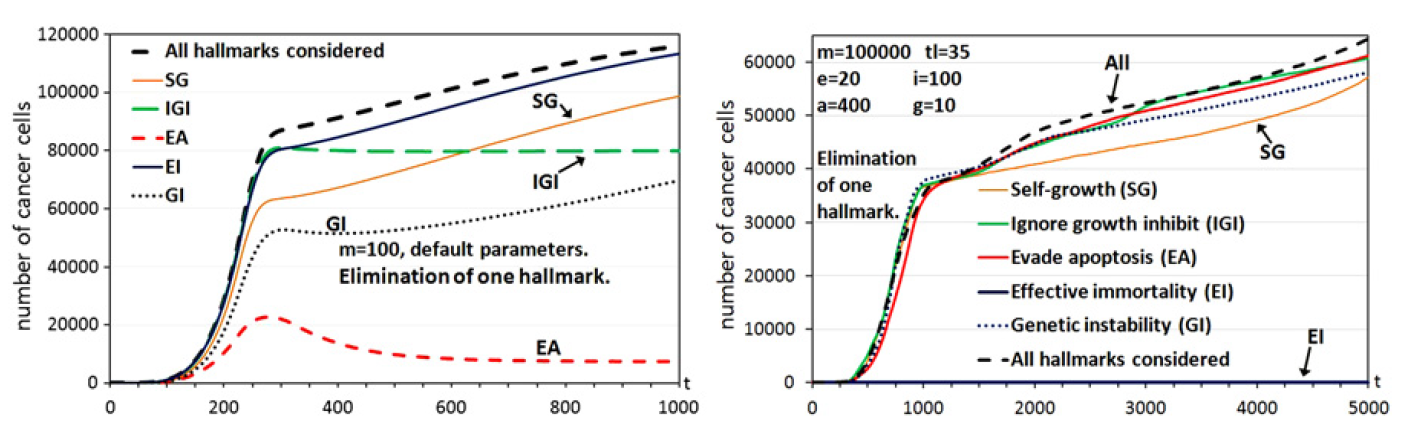
\includegraphics[scale=0.5]{figures/experiments/exp6}
\caption{Resultados de la simulaciones con la eliminación de algún marcador con dos configuraciones diferentes.}
\label{fig:exp6}
\end{figure}
